% ============================================================================
% CAPÍTULO 3 — TRABALHOS RELACIONADOS
% ============================================================================

\chapter{Trabalhos Relacionados}
\label{cap:trabalhos}

Nesta seção, são apresentados e analisados trabalhos recentes da literatura que, assim como este projeto, propõem soluções computacionais para a montagem de genomas de organelas. O objetivo desta análise comparativa é contextualizar a presente proposta no estado da arte da área, identificando as abordagens metodológicas existentes e destacando os diferenciais e a contribuição original do pipeline a ser desenvolvido neste trabalho.

\section{MitoHiFi: Montagem com Leituras Longas}

Um trabalho de destaque na área é o MitoHiFi, um pipeline desenvolvido para a montagem de genomas mitocondriais a partir de dados de \textbf{leituras longas} de alta fidelidade (PacBio HiFi --- tecnologia que produz leituras de milhares de pares de bases com alta precisão, em contraste com as leituras curtas de 100--300 bp geradas pela plataforma Illumina). Proposto por \citeonline{ulianosilva2023}, o objetivo principal era criar um método que aproveitasse a extensão e a precisão deste tipo de dado para gerar mitogenomas completos e corretamente circularizados com maior eficiência. A metodologia do MitoHiFi integra ferramentas como o \textit{hifiasm-meta} para montagem e o GetOrganelle para a etapa de finalização, sendo orquestrada por meio de scripts em Shell e utilizando \textbf{Conda} (gerenciador de pacotes e ambientes, alternativa ao Docker para gestão de dependências de software) para o gerenciamento das dependências.

A abordagem do MitoHiFi é extremamente atual por focar em uma tecnologia de sequenciamento de ponta. Seus resultados são expressivos: o pipeline foi utilizado para montar 374 mitogenomas (368 Metazoa e 6 Fungi) em projetos como o Darwin Tree of Life, o Vertebrate Genomes Project e o Aquatic Symbiosis Genome Project, além de identificar automaticamente variantes decorrentes de heteroplasmia e inserções nucleares de sequências mitocondriais (NUMTs) \cite{ulianosilva2023}. No entanto, sua implementação via scripts e Conda, embora eficaz para seu propósito, pode apresentar limitações de portabilidade e reprodutibilidade quando comparada a soluções baseadas em containers e sistemas de workflow. O diferencial do presente TCC reside precisamente neste ponto: enquanto o MitoHiFi inova na aplicação de um novo tipo de dado biológico, nossa proposta foca em uma arquitetura de software mais robusta, utilizando Docker e Nextflow, para garantir que o pipeline de montagem (baseado em leituras curtas) seja universalmente reprodutível e portável.

\section{MITObim: Estratégia de \textit{Baiting and Iterative \mbox{Mapping}}}

O MITObim, desenvolvido por \citeonline{hahn2013}, foi um dos primeiros métodos amplamente utilizados para montagem de organelas a partir de dados de NGS. Sua estratégia de \textit{baiting and iterative mapping} (captura e mapeamento iterativo) consiste em iniciar o processo com uma sequência guia (um fragmento do genoma alvo ou de uma espécie próxima) e, a partir dela, recuperar leituras homólogas (isto é, leituras suficientemente similares à sequência guia para corresponderem ao genoma mitocondrial), refinando o alinhamento de forma iterativa até a montagem completa do mitogenoma.

Em testes com dados reais de NGS, o MITObim demonstrou capacidade de recuperar mitogenomas completos com acurácia superior a 99,5\% em menos de 24 horas utilizando um computador desktop padrão \cite{hahn2013}. Apesar desses resultados e de sua relevância histórica como pioneiro na abordagem, o MITObim apresenta limitações em termos de eficiência computacional e escalabilidade, especialmente quando aplicado a conjuntos de dados maiores ou de maior complexidade, vindo a ser gradualmente substituído por ferramentas mais modernas, como o NOVOPlasty e o GetOrganelle.

\section{GetOrganelle: Montagem Baseada em Grafos}

O GetOrganelle, proposto por \citeonline{jin2020}, é uma das ferramentas mais recentes e populares para montagem de organelas. Ele utiliza \textbf{grafos de montagem} (estruturas matemáticas em que os nós representam fragmentos de sequência e as arestas representam sobreposições entre eles) derivados de dados de NGS para isolar e reconstruir genomas de organelas, oferecendo resultados robustos tanto para mitocôndrias quanto para cloroplastos (organelas fotossintetizantes de plantas). Em uma avaliação sistemática com 50 datasets publicados de plantas, o GetOrganelle foi capaz de remontar plastomas circulares em 47 dos 50 casos --- uma taxa de sucesso significativamente superior à do NOVOPlasty. Além disso, a avaliação por mapeamento de reads demonstrou que os plastomas montados pelo GetOrganelle são geralmente mais acurados que os publicados originalmente ou remontados pelo NOVOPlasty \cite{jin2020}. A ferramenta tem se destacado também por sua capacidade de gerar todas as configurações possíveis quando os genomas apresentam configurações \textit{flip-flop} ou outros isômeros mediados por repetições, oferecendo resultados consistentes mesmo em organismos com maior complexidade genômica.

No entanto, assim como outras ferramentas tradicionais, o GetOrganelle depende de um ambiente de software adequado para ser executado, geralmente configurado manualmente pelo usuário ou via gerenciadores como Conda, o que ainda pode limitar sua reprodutibilidade plena em diferentes contextos computacionais. Cabe notar que, embora o GetOrganelle apresente taxas de sucesso e acurácia superiores ao NOVOPlasty em plastomas de plantas, a literatura recente demonstra que o NOVOPlasty permanece como a ferramenta predominante para montagem de mitogenomas de metazoários --- sendo adotado em estudos recentes de larga escala com 213 mitogenomas de lagartos \cite{zhan2024} e em trabalhos individuais de peixes, arraias, moluscos e invertebrados \cite{kundu2024,guerreiro2025,shi2024,tao2024}. Essa preferência pela comunidade reforça a escolha do NOVOPlasty como montador neste pipeline.

\section{MToolBox: Foco em Genomas Mitocondriais Humanos}

O MToolBox, apresentado por \citeonline{calabrese2014}, foi uma das primeiras pipelines integradas voltadas especificamente para o estudo de genomas mitocondriais humanos. Ele combina montagem, anotação e análise funcional em um único fluxo, permitindo identificar \textbf{variantes mitocondriais} (alterações pontuais na sequência de DNA que distinguem indivíduos ou populações) relevantes para estudos biomédicos e populacionais.

Apesar de sua contribuição para o campo, o MToolBox é fortemente orientado ao contexto humano e não é tão amplamente aplicável a outros organismos. Além disso, por ter sido desenvolvido antes da adoção massiva de containers e workflows, carece de recursos de portabilidade e reprodutibilidade presentes em soluções mais modernas.

\section{MitoZ: Pipeline Integrado para Metazoários}

O MitoZ, proposto por \citeonline{meng2019}, é um toolkit que integra as etapas de montagem \textit{de novo}, anotação e visualização de genomas mitocondriais de animais em um único fluxo de trabalho. Internamente, o MitoZ utiliza o montador MEGAHIT para a montagem, o programa \texttt{cmsearch} (da suíte Infernal) para predição de tRNAs baseada em modelos de covariância, e gera automaticamente mapas circulares do mitogenoma. Em benchmarks com 50 amostras, o MitoZ demonstrou capacidade de recuperar mais mitogenomas completos e com maior acurácia que o NOVOPlasty isolado (similaridade $>$97\% com referências Sanger para a maioria dos genes) \cite{meng2019}.

Uma vantagem relevante do MitoZ é a disponibilidade de imagem Docker oficial e suporte a Singularity, além da instalação via Bioconda. No entanto, a ferramenta não utiliza um gerenciador de workflow (como Nextflow ou Snakemake), sendo executada como um pipeline monolítico em Python/Shell. Além disso, é restrita a genomas mitocondriais de \textbf{animais}, não oferecendo suporte a plastomas ou outros organismos. Os desenvolvedores recomendam limitar os dados de entrada a aproximadamente 0,3\,Gbp, pois volumes excessivos podem impedir a circularização.

\section{MitoFinder: Extração em Larga Escala}

O MitoFinder, desenvolvido por \citeonline{allio2020}, foi projetado para extração automatizada e em larga escala de dados mitogenômicos, especialmente a partir de bibliotecas de captura por enriquecimento de alvos (UCE --- \textit{Ultraconserved Elements}), embora também seja aplicável a dados de sequenciamento de genoma completo. A ferramenta oferece flexibilidade na escolha do montador (MEGAHIT, MetaSPAdes ou IDBA-UD) e realiza a anotação de genes codificadores e rRNAs via BLAST contra um genoma de referência fornecido pelo usuário, com predição de tRNAs por MiTFi, ARWEN ou tRNAscan-SE.

Em estudo com 501 bibliotecas UCE de formigas (Formicidae), o MitoFinder recuperou 296 mitogenomas em contig único \cite{allio2020}, demonstrando sua capacidade para processamento em lote. A ferramenta possui ampla generalidade taxonômica, suportando diversos códigos genéticos do NCBI, e gera arquivos em formato GenBank prontos para submissão. Contudo, o MitoFinder foi implementado em \textbf{Python 2.7} (versão já em fim de vida), o que dificulta a instalação, e disponibiliza apenas imagem Singularity (sem Docker oficial). Assim como o MitoZ, não utiliza gerenciador de workflow.

\section{NOVOPlasty: Estratégia \textit{Seed-and-Extend}}

O NOVOPlasty, descrito por \citeonline{dierckxsens2017}, é atualmente uma das ferramentas mais utilizadas para montagem de genomas mitocondriais e cloroplastidiais a partir de dados de NGS de leituras curtas. Baseado na estratégia \textit{seed-and-extend}, o programa inicia a montagem a partir de uma sequência semente fornecida pelo usuário e estende iterativamente o genoma até que a molécula circular esteja completa. Sua popularidade decorre da facilidade de uso e da capacidade de gerar montagens confiáveis mesmo a partir de dados de genoma total. A eficácia do NOVOPlasty em aplicações de larga escala foi recentemente demonstrada por \citeonline{zhan2024}, que utilizaram a ferramenta para montar 213 mitogenomas de lagartos (Squamata), combinando-a com o MITOS2 para anotação funcional --- exatamente a mesma combinação de ferramentas adotada neste trabalho.

No entanto, o NOVOPlasty, como software isolado, ainda demanda configuração manual do ambiente e execução direta pelo usuário, o que pode dificultar sua integração em fluxos mais complexos e comprometer a reprodutibilidade quando diferentes versões ou configurações são utilizadas. É justamente neste ponto que se insere o presente TCC: ao invés de propor um novo montador, o objetivo é integrar o NOVOPlasty em um ecossistema de containers e workflow (Docker + Nextflow), assegurando que seu uso seja portável, automatizado e reprodutível em diferentes ambientes de execução.

\section{Análise Comparativa}

A Tabela~\ref{tab:comparativa} sintetiza as características das ferramentas e pipelines analisados, confrontando-as com a proposta deste trabalho. A comparação considera critérios relevantes para a reprodutibilidade, portabilidade e completude do fluxo analítico.

\begin{table}[H]
\centering
\caption{Comparação entre ferramentas de montagem de organelas e o pipeline proposto.}
\label{tab:comparativa}
\footnotesize
\resizebox{\textwidth}{!}{%
\begin{tabular}{@{}lcccccccc@{}}
\toprule
\textbf{Critério} & \textbf{MitoHiFi} & \textbf{MITObim} & \textbf{GetOrganelle} & \textbf{MToolBox} & \textbf{MitoZ} & \textbf{MitoFinder} & \textbf{NOVOPlasty} & \textbf{Este trabalho} \\
\midrule
Tipo de dado & Long reads & Short reads & Short/Long & Short reads & Short reads & Short reads & Short reads & Short reads \\
 & (HiFi) & & reads & & & & & \\
\addlinespace
Montagem & \checkmark & \checkmark & \checkmark & \checkmark & \checkmark & \checkmark & \checkmark & \checkmark \\
\addlinespace
Anotação funcional & --- & --- & --- & \checkmark & \checkmark & \checkmark & --- & \checkmark \\
 & & & & (humano) & (animais) & (referência) & & (metazoários) \\
\addlinespace
Visualização & --- & --- & --- & --- & \checkmark & --- & --- & \checkmark \\
(mapa circular) & & & & & & & & (Biopython) \\
\addlinespace
GenBank Flat File & --- & --- & --- & --- & --- & \checkmark & --- & \checkmark \\
\addlinespace
Containerização & Parcial & --- & Conda & --- & Docker/ & Singularity & --- & Docker \\
 & (Conda) & & & & Singularity & & & (5 imagens) \\
\addlinespace
Workflow manager & --- & --- & --- & --- & --- & --- & --- & Nextflow DSL2 \\
\addlinespace
Pilot QC automático & --- & --- & --- & --- & --- & --- & --- & \checkmark \\
\addlinespace
Estrutura secundária & --- & --- & --- & --- & --- & --- & --- & \checkmark \\
RNA & & & & & & & & (ViennaRNA) \\
\addlinespace
Execução em laptop & Requer & Servidor & Servidor & Desktop/ & Desktop & Desktop & Desktop & \checkmark \\
 & cluster/HPC & recomendado & recomendado & servidor & & & & (notebook 16 GB) \\
\addlinespace
Código aberto & \checkmark & \checkmark & \checkmark & \checkmark & \checkmark & \checkmark & \checkmark & \checkmark \\
\bottomrule
\end{tabular}}%
\end{table}

A análise comparativa evidencia que, embora cada ferramenta contribua com inovações relevantes para domínios específicos, nenhuma oferece um fluxo integrado que cubra todas as etapas --- desde a aquisição dos dados brutos até a geração de arquivos prontos para submissão ao GenBank --- em um ambiente completamente containerizado e orquestrado. Adicionalmente, nenhuma das soluções analisadas incorpora mecanismos de redução automática do volume de dados (como o Pilot QC e o truncamento adaptativo), o que as torna dependentes de hardware com grande capacidade de armazenamento e memória. A proposta deste trabalho preenche essas lacunas ao combinar montagem, anotação funcional, geração de entregáveis, práticas de reprodutibilidade e acessibilidade computacional em um único pipeline modular, executável em computadores pessoais.

% [SUGESTÃO DE FIGURA]: Gráfico radar comparando as ferramentas

Para complementar a análise tabular, a Figura~\ref{fig:radar_comparativo} apresenta uma visualização em gráfico radar que sintetiza o desempenho relativo de cada ferramenta em cinco eixos qualitativos, pontuados em escala de 1 a 5 conforme os critérios da Tabela~\ref{tab:scores_radar}. Essa pontuação foi atribuída com base nas informações publicadas nos artigos originais de cada ferramenta e na análise direta da documentação e dos repositórios oficiais.

\begin{table}[H]
\centering
\caption{Critérios de pontuação do gráfico radar comparativo (escala 1--5).}
\label{tab:scores_radar}
\footnotesize
\resizebox{\textwidth}{!}{%
\begin{tabular}{@{}lp{10cm}@{}}
\toprule
\textbf{Eixo} & \textbf{Critério de pontuação} \\
\midrule
Reprodutibilidade & Nível de isolamento do ambiente: 1 = instalação manual; 2 = Conda; 3 = Conda + versões pinadas; 4 = Docker ou Singularity; 5 = Docker + workflow manager com versões pinadas \\
\addlinespace
Completude do fluxo & Número de etapas cobertas: 1 = apenas montagem; 2 = montagem + anotação parcial; 3 = montagem + anotação completa; 4 = inclui visualização ou conversão de formatos; 5 = fluxo completo (aquisição → montagem → anotação → entregáveis GenBank) \\
\addlinespace
Acessibilidade computacional & Requisitos de hardware: 1 = requer cluster/HPC; 2 = servidor dedicado recomendado; 3 = desktop padrão; 4 = desktop com dados reduzidos manualmente; 5 = notebook com redução automática de dados \\
\addlinespace
Automação & Grau de intervenção do usuário: 1 = configuração manual extensiva; 2 = scripts isolados; 3 = pipeline com parâmetros manuais; 4 = pipeline com defaults razoáveis; 5 = execução com um único comando + decisões automáticas (Pilot QC, fallback k-mer) \\
\addlinespace
Generalidade taxonômica & Escopo de organismos: 1 = uma espécie (e.g., humano); 2 = um grupo taxonômico restrito; 3 = metazoários; 4 = metazoários + outros eucariotos; 5 = qualquer organismo com genoma mitocondrial \\
\bottomrule
\end{tabular}}%
\end{table}

\begin{figure}[H]
    \centering
    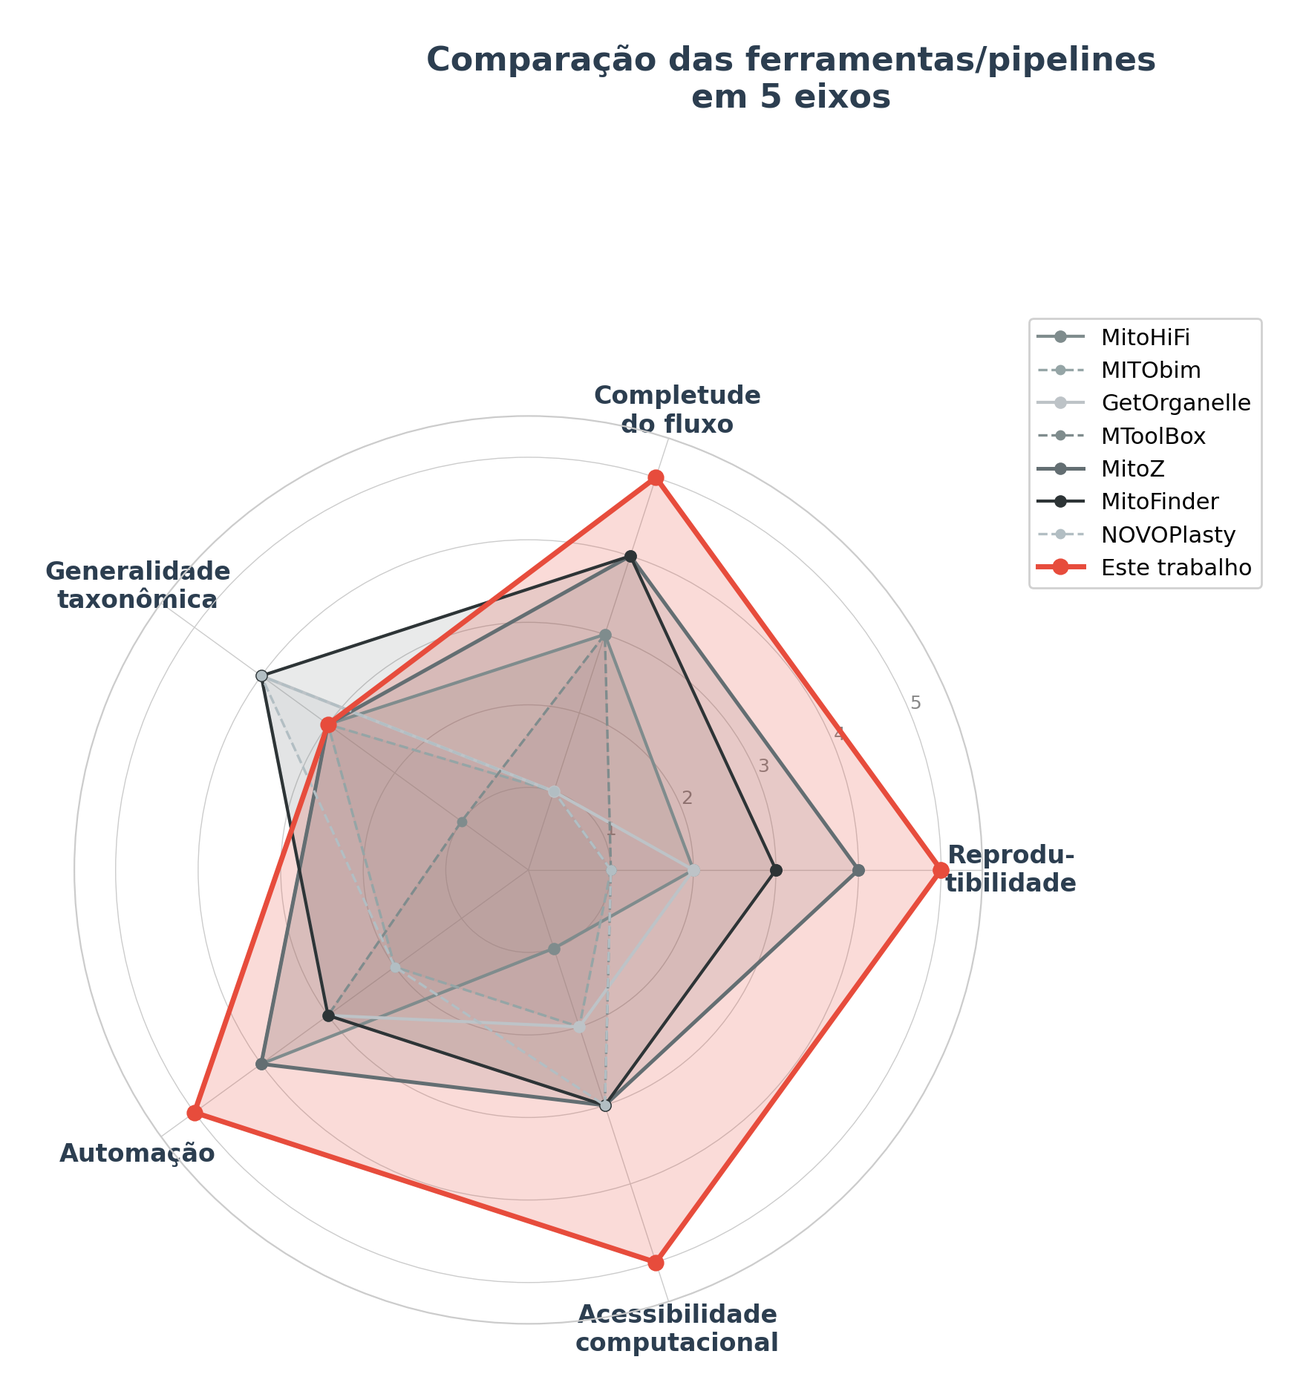
\includegraphics[width=0.80\textwidth]{imagens/radar_comparativo.png}
    \caption{Gráfico radar comparando as ferramentas analisadas em cinco eixos: completude do fluxo, reprodutibilidade, acessibilidade computacional, automação e generalidade taxonômica. A pontuação de cada eixo segue os critérios da Tabela~\ref{tab:scores_radar}.}
    \label{fig:radar_comparativo}
\end{figure}

A análise dos trabalhos relacionados permitiu identificar diferentes abordagens para a montagem de organelas, incluindo pipelines baseados em leituras longas, estratégias iterativas e montadores especializados como o NOVOPlasty. Embora cada solução apresente contribuições relevantes, permanecem lacunas quanto à padronização, portabilidade, completude do fluxo analítico e reprodutibilidade. Nesse contexto, o Capítulo~\ref{cap:metodologia} descreve a metodologia adotada neste trabalho, detalhando a concepção do pipeline proposto e as ferramentas que o compõem.
